\documentclass[12pt]{article} 
\usepackage{amsfonts, amsmath, amssymb} 
\usepackage{dcolumn, multirow} 
\usepackage{setspace} 
\usepackage{epsfig, subfigure, subfloat, graphicx}
\usepackage{booktabs}
\usepackage{tabularx} 
\usepackage{anysize, indentfirst, setspace} 
\usepackage{verbatim, rotating, paralist}
% \usepackage{pdfsync} 
\usepackage{latexsym} 
\usepackage{amsthm} 
\usepackage{fullpage} 
\usepackage{longtable} 
\usepackage{natbib} 
\usepackage{graphicx} 
\usepackage{mathabx} 
\usepackage{txfonts} 
\usepackage{amsfonts} 
\usepackage{parskip} 
\usepackage{stmaryrd} 
\usepackage{mathrsfs} 
\usepackage{dsfont} 
\usepackage{comment} 
\usepackage{url} 
\usepackage{rotating} 
\usepackage{appendix}
\usepackage[capposition=top]{floatrow}

\usepackage[margin=2.5cm]{geometry}

\title{The Illusion of Primary School Dominance in Rural Pakistan}
\author{Nick Eubank}
\date{\today}

\setcounter{tocdepth}{2}

% This is the beginning of a real document!
\begin{document} 
\maketitle

Developing countries -- particularly those in South Asia -- have experienced explosive growth in the rural private schools. Even after controlling for a multitude of observable student characteristics -- including household wealth, and the educational attainment of parents -- private schools deliver superior outcomes to government schools. 

A close examination of the inner workings of private schools provides reason to believe this advantage is well earned, and that private schools may have much to teach government administrators. Private schools pay their teachers on the basis of performance -- providing a strong incentive for teachers to give their best -- and fire teachers who do not perform. Government schools, by contrast, pay their teachers formulaically based on their years in service and their academic credentials (which appear unrelated to teacher effectiveness), and never fire teachers.  

Yet while even the most sophisticated econometric methods available suggest that private schools outperform government schools, these studies remain plagued by problems of selection -- even techniques like ``value-added'' estimation cannot fully address the possibility that school choice is driven by unobservable factors that are correlated with educational attainment. 

This paper makes the case that a large share of the superior performance of private schools that appears in value-added analyses is the result of parents sending their more promising children to private schools. This is shown by exploiting variation in this ``selection'' of high talent children into private schools caused by intra-village caste politics. In particular, this paper argues that in homogenous villages parents send their most intelligent children to private schools, paying private school fees only when they view their children as having significant academic potential. In ethnically fractionalized villages, however, this sorting is disrupted by the desire of high status parents to send their children to private schools regardless of their perceived potential in order to keep them segregated from lower castes. Thus by comparing homogenous villages (with strong selection on academic potential) with fractionalized villages (where this sorting is at least partially disrupted), this paper argues we can place a lower bound on the contribution of sorting to private school performance. 

It is worth noting that this analysis cannot rule out the possibility that private schools do fundamentally outperform government schools. Even in homogenous villages private school students outperform government school students. But by showing the large contribution of sorting to private school performance -- the private-government test-score gap is halved moving from homogenous to heterogeneous villages even after controlling for a plethora of observables in a panel setting -- this paper provides a large, empirical  ``lower bound'' to the importance of sorting which should give analysts pause when examining other empirical results that claim to fully control for sorting. 

This paper is organized out as follows: Section~\ref{overview} provides an overview of the Pakistani context in which this study takes places, including a more detailed discussion of past work. Section~\ref{caste} discusses the social politics of caste in Pakistan. Section~\ref{data} provides an overview of the data and methods employed in this analysis. Section~\ref{selection} shows that as fractionalization increases, school choice becomes less about academic potential and more about social segregation, and Section~\ref{results} shows that this shift causes private and government school test scores to converge. Section~\ref{distance} provides some additional evidence that a significant portion of private school performance is driven by selection, and finally Section~\ref{conclusion} concludes. 

\section{Background -- Public and Private Schools in Rural Punjab}\label{overview}

The last decade have seen an explosion in small, secular private schools in rural Pakistan. According to one World Bank report, ``[b]etween 2000 and 2005, the number of private schools in Pakistan increased from 32,000 to 47,000 and by the end of 2005, one in every 3 enrolled children at the primary level was studying in a private school.'' \citep[p. vi]{Andrabi:2007we}. Although initially met with skepticism among policy makers concerned that private schools would widen the disparity between the economic haves and have-nots, a recent wave of studies has shown that these private schools not only serve a broad portion of the population -- including many poor children from uneducated homes -- but that they also appear to be delivering educational outcomes that are markedly superior to their government school counterparts. 

The most detailed existing data on private schools in Pakistan comes from an analysis of national school surveys by \cite{Andrabi:2008ji}, who find that villages with private schools have higher enrollment rates, especially among girls. Further, they find that private schools are exceptionally affordable, even to poor families. They report that ``[i]n rural areas, the median annual fee translates into \$1.50 a month, or less than a dime a day,'' making private school potentially affordable even to those living below the dollar-a-day poverty line. The average rural tuition fee in Punjab -- home to more than half of Pakistan's primary-school-aged children -- represents less than 1.7\% of average household expenditures. As a result, while private school students tend to be wealthier and better educated than government school counterparts, the distributions overlap tremendously as shown in Figure~\ref{overlapwealtheduc}, reprinted from a World Bank survey of schools in 112 villages in rural Punjab.

\begin{figure}[htb]
	\begin{center}
	\caption{Government and Private School Student Demographics}\label{overlapwealtheduc}
	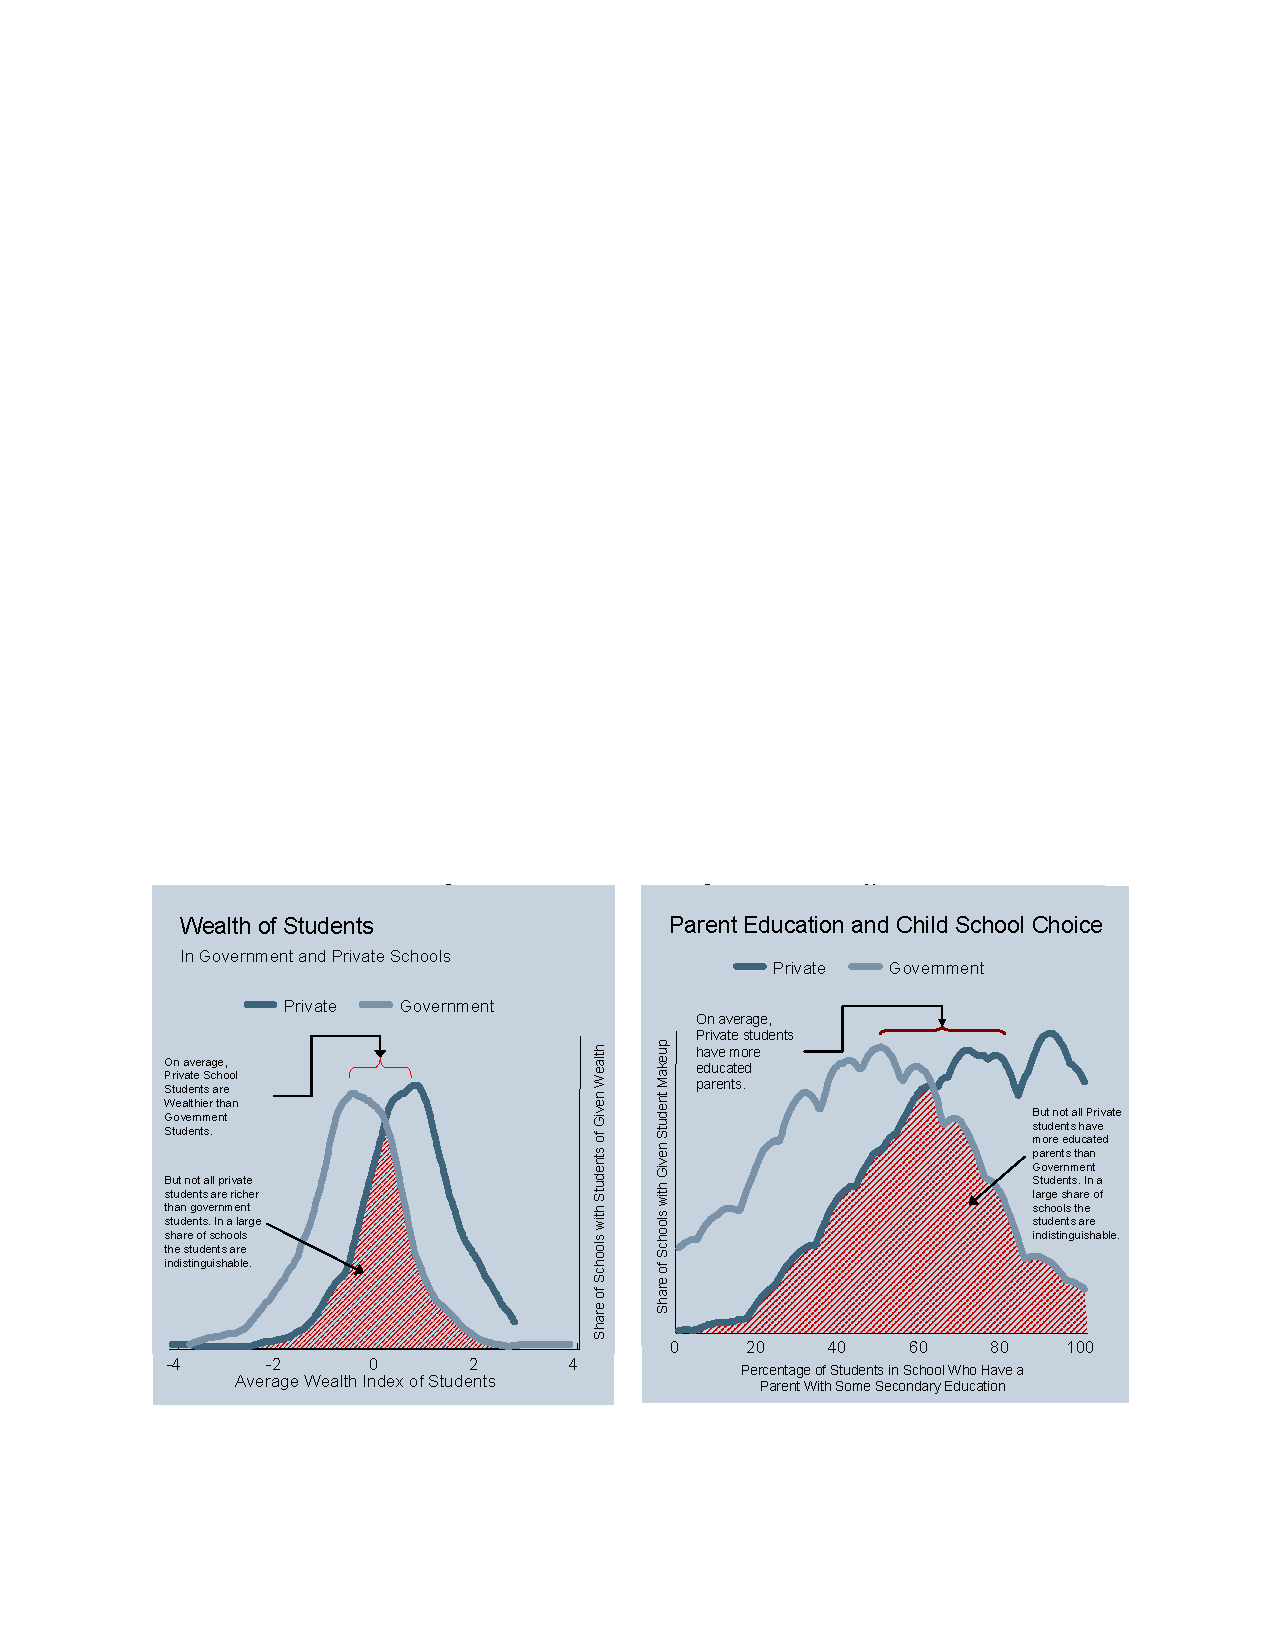
\includegraphics[scale=1.0]{graphs/distributional_overlap.pdf}
	\floatfoot{Reprinted from \citep[p. 51]{Andrabi:2007we}}
	\end{center}
\end{figure}

Nor is this pattern unique to Pakistan. Similar growth in private schools has also been observed in India. [MORE TO BE INCLUDED HERE]

More promising than the potential contribution of these private school to higher enrollments, however, its their potential contribution to improved educational attainment. Even controlling for all observable child characteristics (like wealth and parental education), private school students still appear to dramatically outperform government school students. Using data from Punjab, Pakistan, \cite{Andrabi:2011hl} find that private schools provide students gain 0.25 standard deviations more per year on test scores on average, a difference of more than a year of schooling. Remarkably, this is accomplished despite the fact that government schools hire better educated and trained teachers and pay them dramatically more than private school teachers. 

In order to better understand this performance differential, in 2003 the World Bank, Harvard University, and Pomona College, in conjunction with the Government of Punjab, mounted a massive four year survey of schools, students, teachers, and households in 112 villages in rural Punjab. The aim of the project -- the Learning and Educational Attainment in Punjab Schools (LEAPS) survey (on which this author was a research assistant) -- was to study the inner workings of government and private schools in the hopes of better understanding how private schools were able to do so much with so little. 

The conclusion of the LEAPS authors is that private schools are able to deliver better educational outcomes despite hiring local women with only secondary educations and no training and paying relatively low wages is that where government schools focus on inputs, private schools are output-oriented. Government schools pay their teachers well, but their pay is unrelated to the performance of their students. Private school teachers, by contrast, are paid more when their students do better. As a result, government school teachers exert less effort. As shown in Figure~\ref{payandabsenteeism} from the report, while frequently absent private school teachers are paid less, absent government school teachers are actually paid \emph{more}, and where private school teachers with high score students are paid more, no such relationship exists for government teachers. This leads the authors to conclude that:

\begin{quotation}
Teacher and institutional attributes can be broadly separated into three categories: hard to observe teacher characteristics such as motivation, which can emerge only over time, easy to observe characteristics such as educational qualifications, experience and training and, the institutional framework embodied in incentives such as the teacher salaries and bonuses. Research in the United States has tried to separate the influence of the first two types of characteristics (motivation and qualification); given that most of this research is for public school teachers, it has made less progress on the impact of incentives. This research finds that characteristics like motivation and a love of teaching are far more important in explaining the variation in student learning compared to educational qualifications, experience, and training. Experience for instance, matters only in the first year. In short, in systems with the same set of incentives, teachers appear to be born, not made.\citep[p. 78]{Andrabi:2007we}
\end{quotation}

\begin{figure}[htb]
	\begin{center}
	\caption{}\label{payandabsenteeism}
	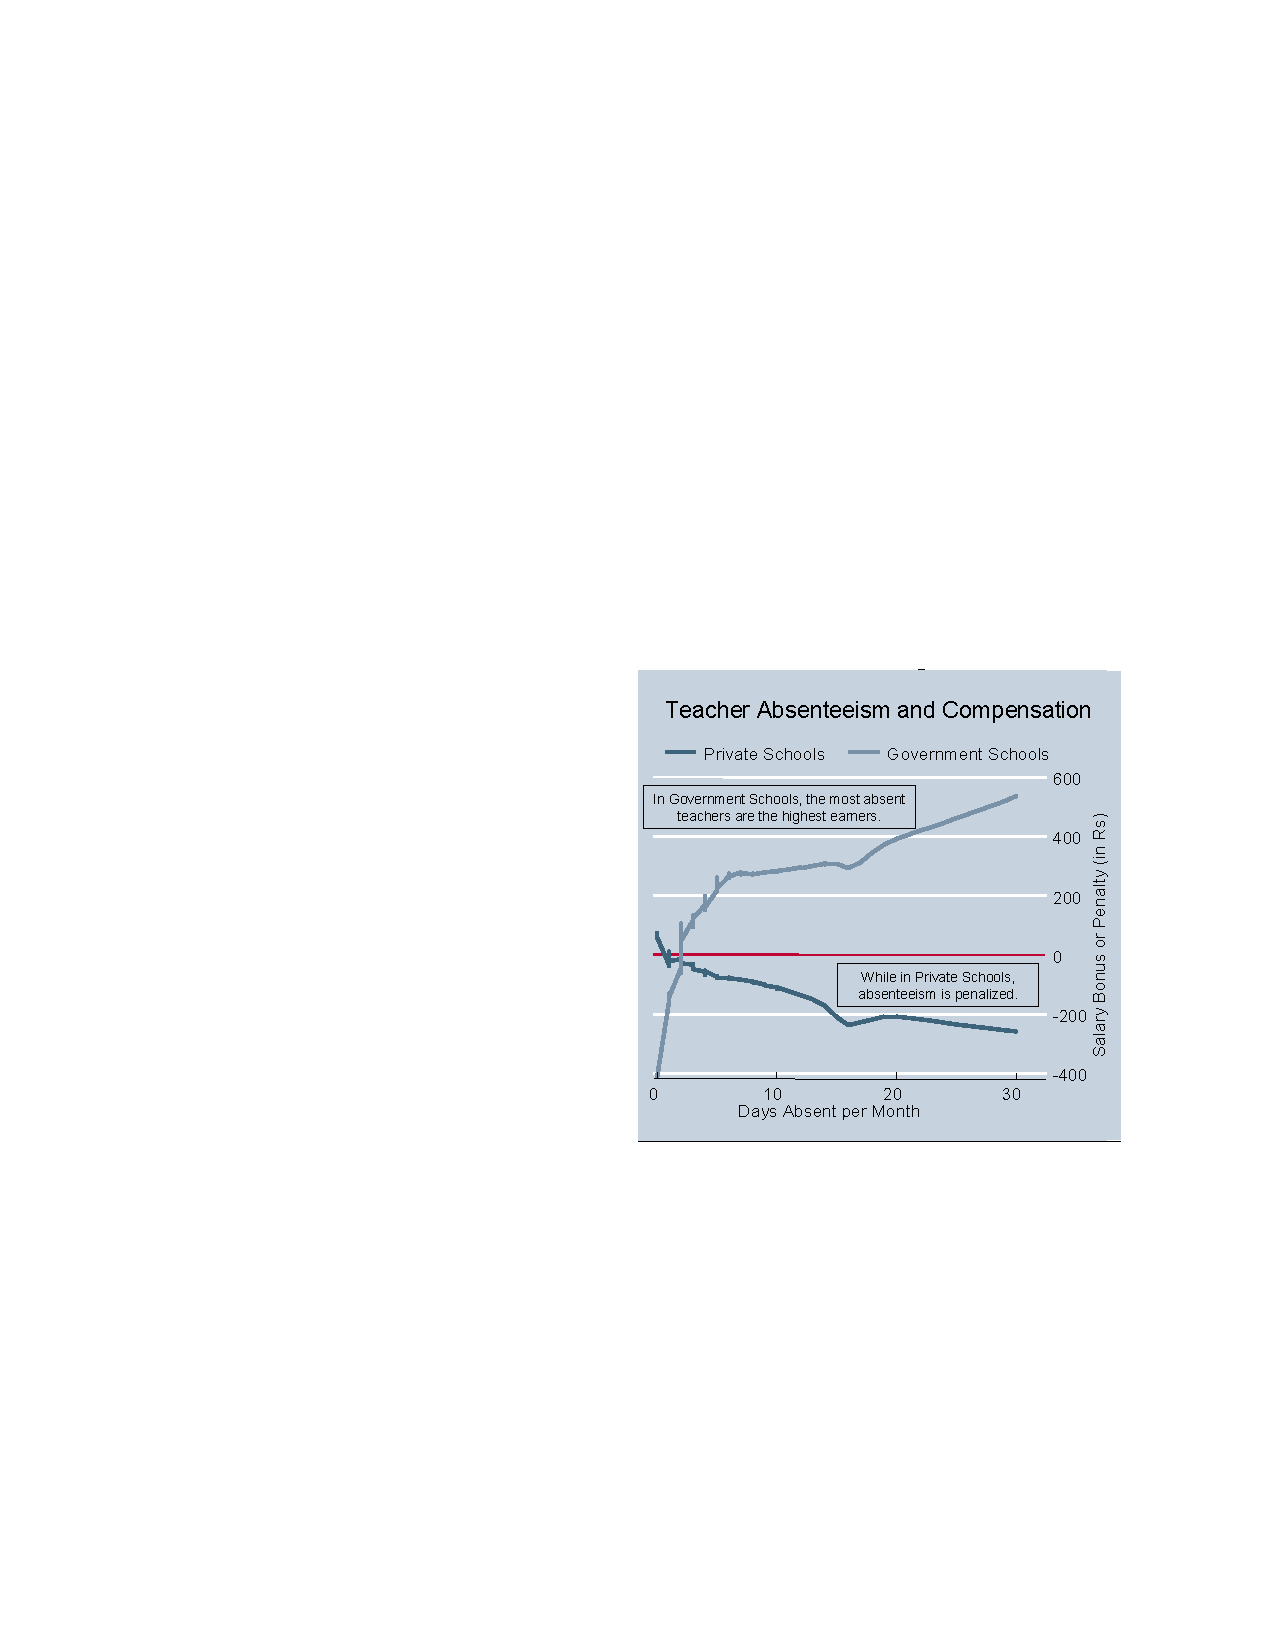
\includegraphics[scale=0.82]{graphs/absenteeism_and_pay.pdf} 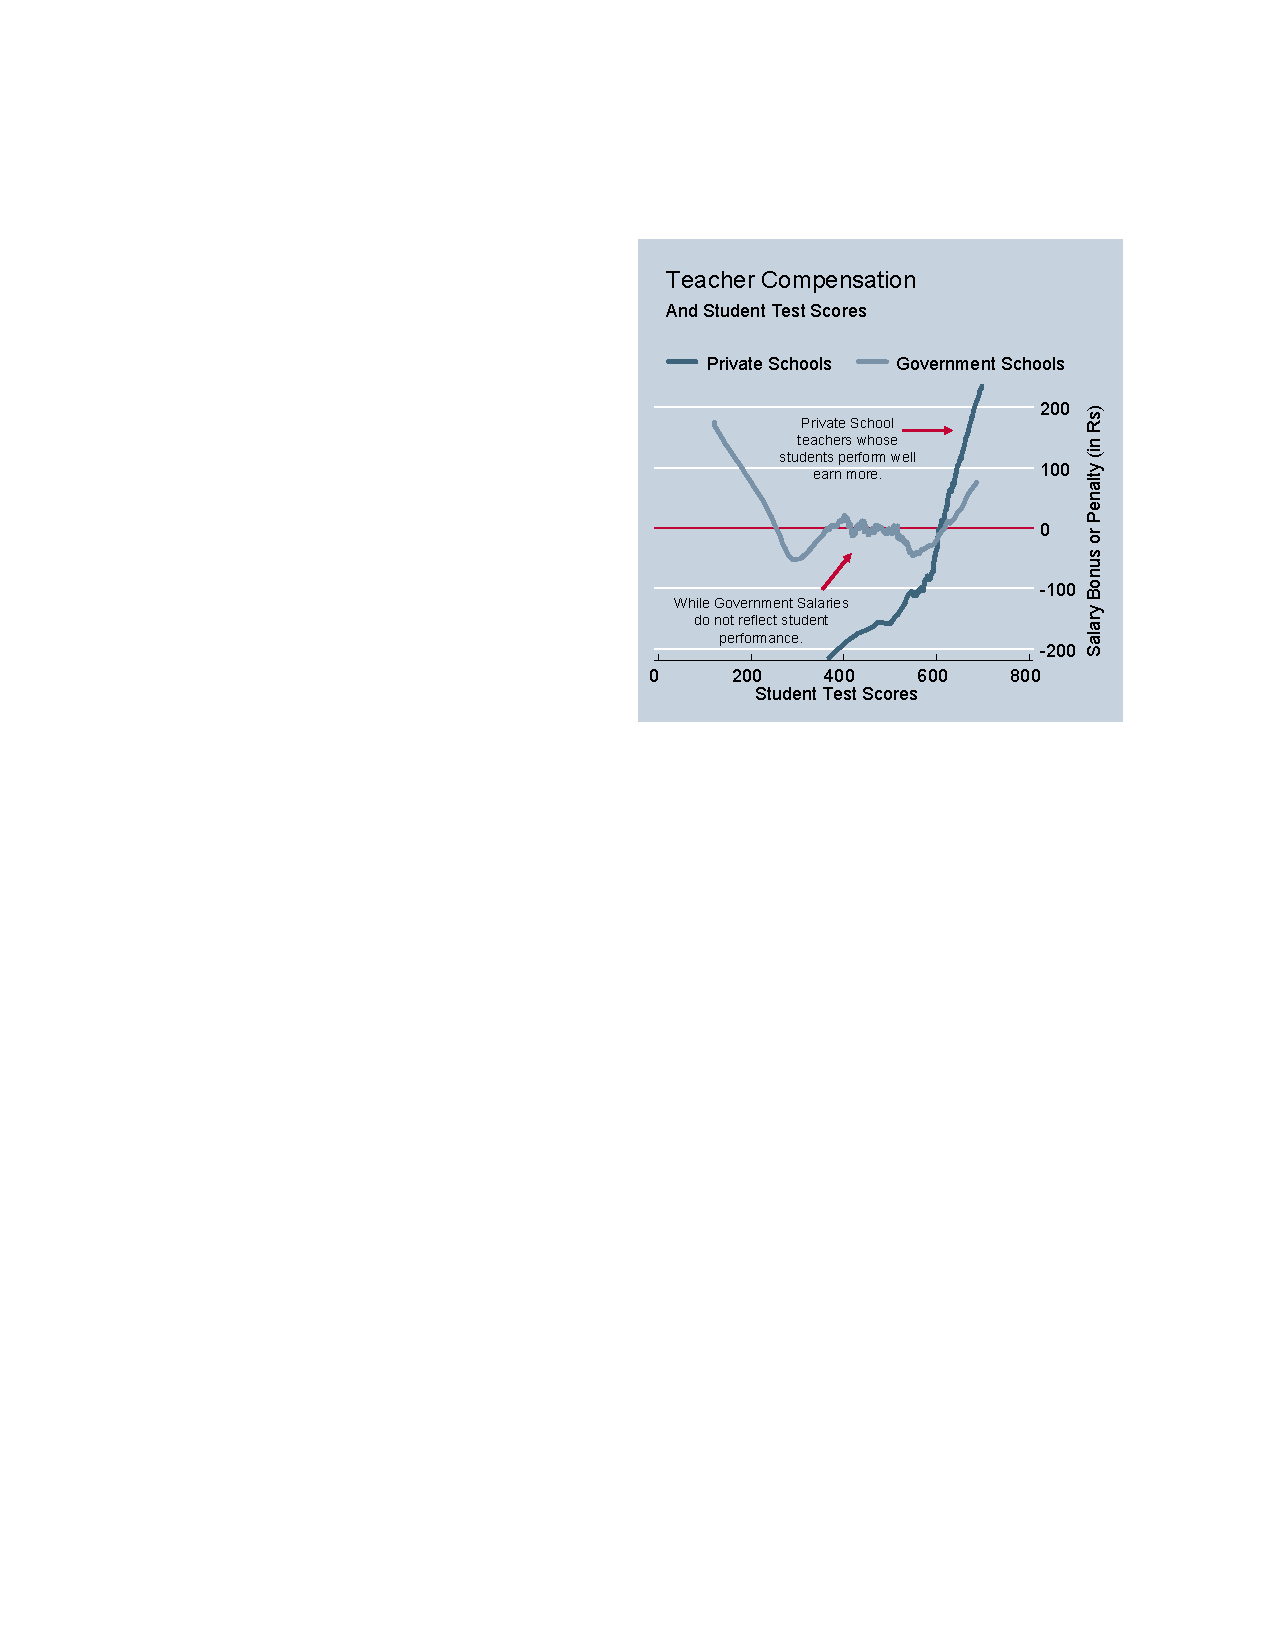
\includegraphics[scale=0.8]{graphs/compensation_scores.pdf}
	\end{center}
\end{figure}

If it is true that private schools outperform government schools in Pakistan despite hiring less educated teachers and paying them dramatically less, then these rural private schools could offer a model of how to improve educational outcomes while potentially spending less. 

Yet the LEAPS study is based on observational data, and while in subsequent work the authors do their best to control for all possible observational contaminants using value-added regressions, dynamic panel specifications, and even an analysis of children who switch schools \citep{Andrabi:2011hl}, selection on unobservables remains a viable alternative explanation for private school performance, and one which this paper contends has likely been under-appreciated. 


\section{Data and Methodology}\label{data}

This analysis is based on panel data from the Learning and Educational Attainment in Punjab Schools (LEAPS) survey, administered jointly by the World Bank, Pomona College, Harvard University, and with the assistance of the Government of Punjab. The LEAPS survey was conducted in 112 villages in the Punjab districts of Attock, Faisalabad, and Rahim Yar Khan annually from 2003-2007. The data consists primarily of two panels of students -- one (initiated in 2003 with an initial population of 12,110 children) which followed students for four years, and one (initiated in 2005 with an initial population of 11,852 students) which followed students for two years. Each panel represents the universe of enrolled students in sample villages in Class 3 in both government and private schools. 

Students in both panels were administered annual exams in English, math, and Urdu. In addition, approximately half of students were administered demographic surveys which include questions on parental education and household wealth. These exams were designed and piloted by the LEAPS team, and subsequently standardized using Item Response Theory methods. The test scores presented here are the normalized IRT results, which have a mean of zero and standard deviation of one among students in Class 3. 

In addition to testing and surveying students, the LEAPS survey also collected data on schools, teachers, and a random sample of 10 households per village with children of school-eligible age. Further, some data were also obtained from a listing census conducted in sample villages prior to the start of the LEAPS survey that include basic demographic information on all households, allowing for the computation of more accurate village level statistics.

\subsection{Measuring Test Scores}\label{}

Test data from the LEAPS survey is analyzed using a lagged value-added model, where current knowledge is assumed to be an additive function of all current and past inputs and a stochastic error term. As past inputs are unavailable, however, they are generally subsumed into a lagged dependent variable included as a control, so that valued-added regressions take the form:
\begin{eqnarray*}
	y_{t}=X_t\beta+y_{t-1}\gamma + \epsilon_t
\end{eqnarray*}
Where X is a vector of child, school, and village controls, and $\gamma$ is assumed to capture all past inputs and unobservable heterogeneity across students. As the interest of this analysis is on the difference between government and private school students, primary interest is on a dummy for school type included in the vector of controls $X$. 

Three aspects of this specification are worth emphasizing. First, while the inclusion of a lagged dependent variable effectively controls for unobserved differences that affect learning \emph{levels}, it cannot control for unobserved heterogeneity that affects \emph{learning} rates. It is for this reason that while superior to other available methods, value-added analyses can not fully overcome selection issues.\footnote{Some analysis have turned to second-differencing the data and focusing on students who change schools, but these analyses have their own limitations, among them limited sample sizes (given that changes between types of school are relatively infrequent in most surveys) and the assumption that school changes are not the result of some unobserved shock (i.e. that school switches are not accompanied by contemporaneous with other changes).}

Second, the $\gamma$ term can be interpreted as the ``persistence parameter,'' in that it estimates the degree to which past learning may carry forward. A value of one is equivalent to assuming that children do not forget past lessons, while a value of zero corresponds to students forgetting all past lessons each year. While imposing a persistence parameter of one may seem reasonable -- it amounts to regressing the difference in test scores from time $t-1$ to time $t$ on controls -- a growing literature suggests that the test score gains of short term interventions often ``die out'' over time, suggesting this is not the case\citep{Glewwe:2010hj,Currie:1995wo,Andrabi:2011hl}, and so this parameter is left flexible. 

Finally, lagged test scores from all three subjects -- English, Urdu, and math -- are included in all specifications to instruments for the primary lagged test score of interest. This helps to minimize the attenuation bias caused by measurement error in past test scores, a problem noted by numerous authors \citep{Kane:2002if,Chay:2005wu,Andrabi:2011hl}. 

For robustness, the primary analysis of this paper is duplicated at the level of the village. To do so, child test scores are regressed on lagged test scores and demographic controls (as above) along with village fixed effects and separate private-school dummies for each village. The difference between the village private-school dummy coefficients and the village dummy coefficients are then extracted as a village-level estimate of the government-private test score gap. These village-level gaps are then regressed against a series of village-level controls, include village fractionalization, wealth, size, land fractionalization, and adult literacy. 

\section{Caste Fractionalization}\label{caste}

Caste -- known variously as \emph{biraderi} or \emph{zaat} -- is a central aspect of rural social identity in Pakistan, especially in Punjab. While biraderi is a somewhat distinct concept from the idea of ``caste'' in India, ``it retains a very important feature of the [Indian subcaste] -- that of an inherent, inbuilt hierarchy that governs social interactions. Society is hierarchically ordered with the Syeds at the top, followed by the landowning castes, then by the service castes or kammis, and finally by the Musallis, who occupy the lowest rung of the social ladder. This ordering dictates much of the social life in a Punjabi village and is most profound in the notions of community cooperation, where solidarity is strongest within a biraderi.''\citep[p. 29]{Gazdar:2007vt}. Further, while Biraderi is correlated with wealth, land holdings, and education, it is not synonymous with economic class. As a related report observes, ``while economic power is required to reinforce biraderi-based dominance, membership of a dominant biraderi can help mitigate some of the effects of being economically poor. As one respondent put it, `the poorest Jatt is still better off than the richest kammi.''' \citep[p. 13]{Gazdar:2007vt} 

While the centrality of caste politics is relatively universal across villages in Punjab, there is significant variation in village \emph{biraderi} composition. Figure~\ref{fracdensities} below shows the density plot of villages of different levels of ethnic fractionalization, as measured by a simple herfindahl index.\footnote{The herfindahl is a common measure of fractionalization equal to the probability that any two randomly selected individuals belong to the same group. Village fractionalization is computed using data from a village census conducted in 2002 to facilitate household sampling for the LEAPS survey which includes data on the biraderi of all households in LEAPS villages. Details of included \emph{biraderis} are presented in Appendix~\ref{biarderis}.} As the figure shows, there is significant variation in the degree of fractionalization both within and across the three districts of the LEAPS survey.

\begin{figure}[htb]
	\begin{center}
	\caption{}\label{fracdensities}
	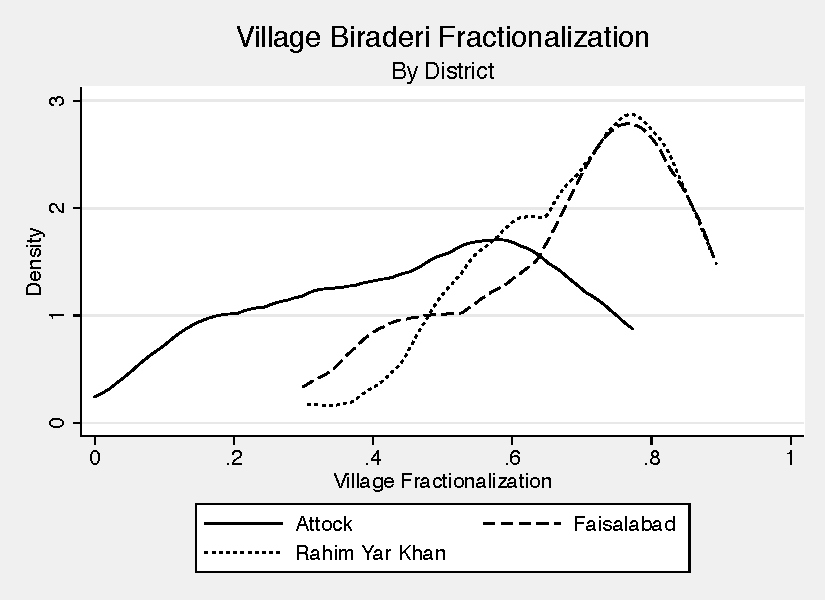
\includegraphics[scale=1.0]{graphs/village_frac_by_district.pdf}
	\end{center}
\end{figure}

Interestingly, segregation is not clearly related to any other village characteristics, as shown below in Table~\ref{vsummary}. Nor is this lack of clear relationship driven by district differences -- as shown in Table~\ref{vsummarydemeaned}, in which summary statistics are computed after demeaning values for district averages. Please note that ``high,'' ``medium'' and ``low'' fractionalization in these tables refer to village fractionalization terciles. [Tables to be reformatted]

% matrix: results file: /Users/Nick/dropbox/data/LEAPS/data//constructed/ethnic_info/docs/tables/village_summary.tex   2 Sep 2012 21:28:58
\begin{table}[htbp]
\caption{\label{vsummary} Village Summary Statistics}\centering\medskip
\begin{tabular}{|l|l|l|l|l|l|}\hline  
 & Median Expend  & Adult Lit Rate  & Pct Enrollment  & Schools per HH  & Num Households  \\ \hline  
Highest Frac &      4967 &        39 &        70 &      .017 &       699 \\ \hline 
Moderate Frac &      4194 &        34 &        67 &      .019 &       631 \\ \hline 
Lowest Fract &      4719 &        38 &        75 &      .011 &       562 \\ \hline 
All &      4641 &        37 &        71 &      .016 &       631 \\ \hline 
  \end{tabular}
\end{table}

% matrix: results file: /Users/Nick/dropbox/data/LEAPS/data//constructed/ethnic_info/docs/tables/village_summary_demeaned.tex   2 Sep 2012 21:29:00
\begin{table}[htbp]
\caption{\label{vsummarydemeaned} Summary Statistics, After Subracting District Averages}\centering\medskip
\begin{tabular}{|l|l|l|l|l|l|}\hline  
 & Median Expend  & Adult Lit Rate  & Pct Enrollment  & Schools per HH  & Num Households  \\ \hline  
Highest Frac &       1.2 &      -.17 &        -1 &     .0019 &        65 \\ \hline 
Moderate Frac &        19 &      -.51 &         1 &    .00041 &       1.4 \\ \hline 
Lowest Fract &       -19 &       .65 &       .12 &    -.0023 &       -68 \\ \hline 
All &  -3.3e-06 &   9.2e-08 &  -1.3e-07 &  -1.3e-11 &  -9.1e-07 \\ \hline 
  \end{tabular}
\end{table}



\section{Selection}\label{selection}

The central argument of this paper is that the criteria by which parents decide whether to send their children to government or private schools varies systematically with village \emph{biraderi} fractionalization. As shown in this section, while parents everywhere are inclined to send children they perceive as being ``more intelligent'' to private schools -- presumably because their strong academic performance will make the cost of private schools worthwhile -- in fractionalized villages parents also take into account the social status of other students in each school. Parents from ``high status'' biraderis in particular tend to send their children to private schools, while ``low status'' children are left concentrated in government schools. 

This variation in the importance of unobserved academic potential in determining school choice is leveraged here. It is important to keep in mind, however, that differences seen between homogeneous and fractionalized villages are best viewed as a lower-bound on the importance of sorting, not a direct estimate of its effect. That is because while diminished, academic potential likely still plays a role in school choice in fractionalized villages. 


\subsection{Role of Intelligence}\label{}

Private schools in rural Punjab are highly affordable, but there is nevertheless strong evidence that parents only choose to bear the cost of private schools when they believe their children have strong academic potential. As shown in Table~\ref{hhselection} below, which regresses the choice to send a child to a private school on a number of characteristics, parental perceptions of child intelligence are an extremely strong predictor of whether a parent will send their child to a private school. Most notably in this table, this pattern holds even \emph{within individual households}. As shown in Column 2, which includes household fixed effects, many parents send the child they perceive to be more intelligent to private school and the child they perceive to be less intelligent to government schools. 

\begin{table}[htbp]\centering
\def\sym#1{\ifmmode^{#1}\else\(^{#1}\)\fi}
\caption{School Choice and Child Intelligence\label{hhselection}}
\begin{tabular}{l*{2}{c}}
\hline\hline
                &\multicolumn{1}{c}{(1)}&\multicolumn{1}{c}{(2)}\\
                &\multicolumn{1}{c}{Village FE}&\multicolumn{1}{c}{HH FE}\\
\hline
Mom Reports Child Above Average Intelligence&    0.056***&    0.041*  \\
                &   (2.70)   &   (1.98)   \\
Mom Has Some Schooling&    0.080   &   -0.034   \\
                &   (1.43)   &  (-0.28)   \\
Dad Has Some Schooling&    0.082***&    0.085   \\
                &   (3.20)   &   (0.72)   \\
PCA Wealth Index&   -0.028   &        .   \\
                &  (-1.25)   &        .   \\
Age             &   -0.019***&   -0.017***\\
                &  (-3.45)   &  (-3.22)   \\
Age Squared     &  0.00025*  &  0.00017   \\
                &   (1.67)   &   (1.61)   \\
Female          &    0.035   &   0.0020   \\
                &   (1.59)   &   (0.07)   \\
\hline
Observations    &     3361   &     3361   \\
\hline\hline
\multicolumn{3}{l}{\footnotesize \textit{t} statistics in parentheses}\\
\multicolumn{3}{l}{\footnotesize * p<0.10, ** p<0.05, *** p<0.01}\\
\end{tabular}
\end{table}


\subsection{Biraderi Segregation}\label{}

Yet intelligence is only one of a number of factors that appear to play into school choice -- schools are also relatively segregated by \emph{biraderi}, and this segregation is especially evident in highly fractionalized villages. Figure~\ref{numcastes} below plots the number of biraderis represented in each school for high, medium, and low fractionalized villages. As the figure shows, despite large differences in the fractionalization of the villages in which these schools operate, a remarkably similar numbers biraderis a present among their student bodies.

\begin{figure}[H]
	\begin{center}
	\caption{}\label{numcastes}
	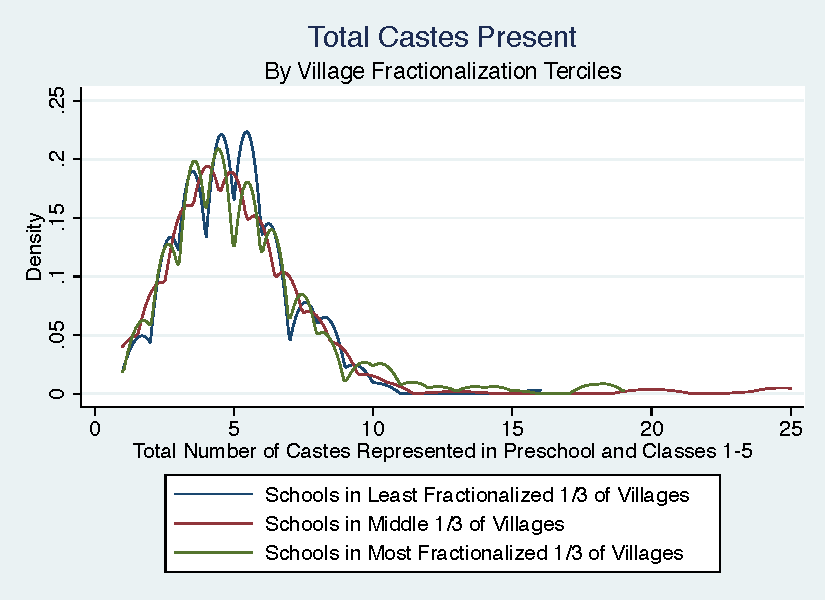
\includegraphics[scale=1.0]{graphs/totalpresent.pdf}
	\end{center}
\end{figure}

This figure is easily interpreted, but does not take into account the relative size of the population of each \emph{biraderi} within the student body. Figure~\ref{toptwo} plots the population share of the two largest biraderis among students in the village at large and in each school level respectively. Again, this figure shows that while in more fractionalized villages the share of students from the top two castes in the average school is indeed slightly lower, it does not come close to keeping pace with changes in village demographics.

\begin{figure}[H]
	\begin{center}
		\caption{Village and School Fractionalization}\label{toptwo}
		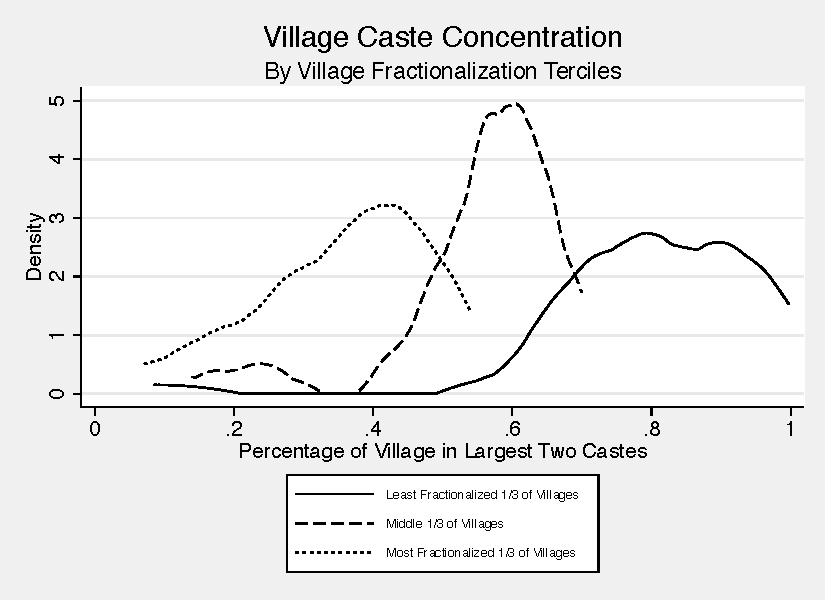
\includegraphics[scale=.6]{graphs/village_toptwo.pdf}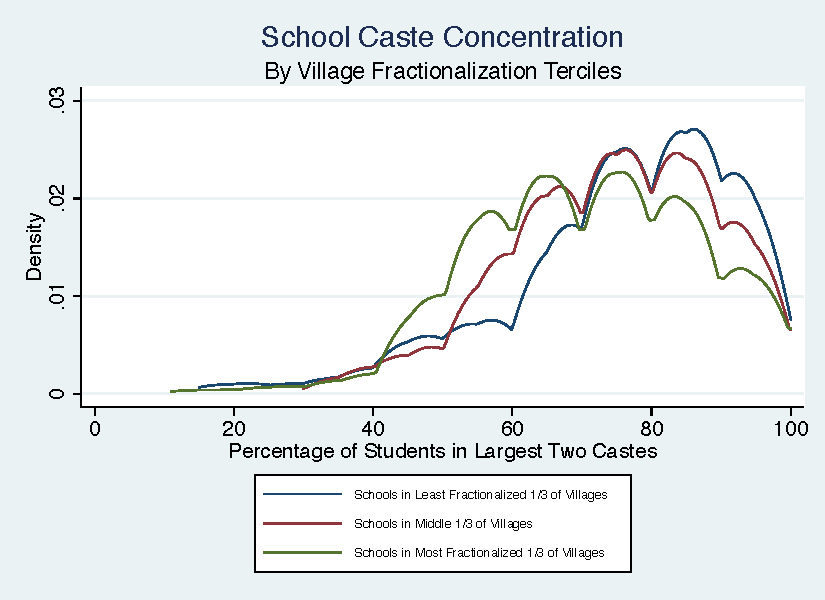
\includegraphics[scale=0.6]{graphs/school_toptwo.pdf}
	\end{center}
\end{figure}

And finally, if schools are unsegregated, then we would expected herfindahl indices computed within each school to track closely with herfindahl indices computed at the village level. Yet as shown in Figure~\ref{schoolvvillageherf}, this is far from the case. Almost all schools are below the 45 degree line that would indicate school and village diversity moving one for one, and many are well below.

\begin{figure}[H]
	\begin{center}
	\caption{}\label{schoolvvillageherf}
	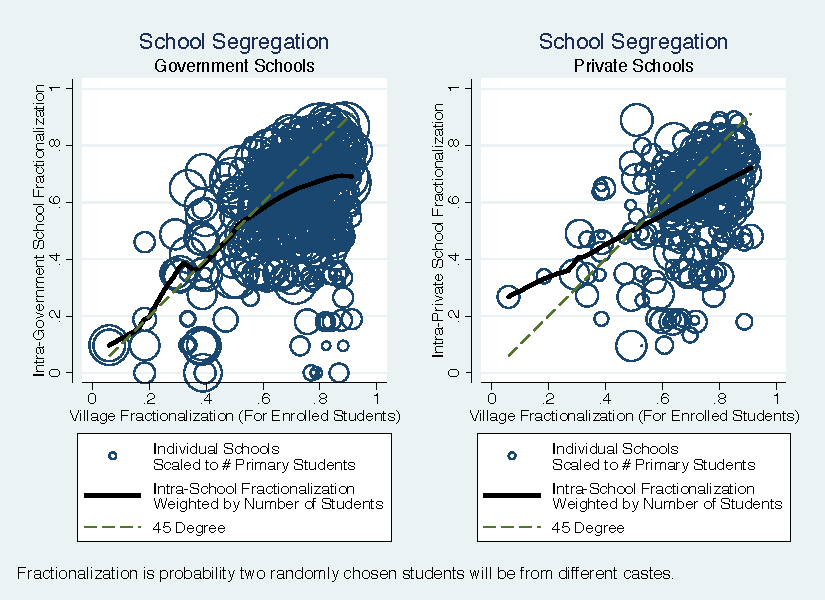
\includegraphics[scale=1.0]{graphs/intra_versus_intervillage_frac_combined.pdf}
	\end{center}
\end{figure}

This data shows a clear pattern of segregation, but it does not provide an entirely clear picture of which groups are attending which schools.  Grouping \emph{biraderis} into ``high'' and ``low'' social status groupings allows for a better understanding of segregation patterns. The crudeness of these categorizations is unfortunate, but necessary -- although \emph{biraderis} are associated with strict hierarchies within villages, there does not exist an explicit global hierarchy of biraderis in Pakistan as in India. As a result, these hierarchies may vary somewhat from village to village, and as noted previously, this variation may not perfectly follow economic position. Fortunately, interviews with numerous Pakistanis has provided evidence that these categorizations are sufficient consistent at this level of generality and in the region of the LEAPS survey for these rankings to be useful.\footnote{Some interviewees have also provided threefold divisions, which generate consistent results with those presented here.} The specific groupings used in this paper can be found in Table~\ref{biraderiranks} in Appendix~\ref{biraderis}.

As shown in Table~\ref{highpooling}, these categorizations make it possible to show that in villages with higher ethnic fractionalization, a larger share of private school students come from higher status \emph{biraderis} and a larger share of government school students come from low biraderis.


\begin{table}[htbp]\centering
\def\sym#1{\ifmmode^{#1}\else\(^{#1}\)\fi}
\caption{Student Social Status by School Type\label{highpooling}}
\begin{tabular}{l*{2}{c}}
\toprule
                &\multicolumn{1}{c}{(1)}&\multicolumn{1}{c}{(2)}\\
                &\multicolumn{1}{c}{Pct of Students High Status}&\multicolumn{1}{c}{Pct of Students High Status}\\
\midrule
Private School  &    -0.11** &    -0.13** \\
                &  (-2.30)   &  (-2.13)   \\
Biraderi Fractionalization&   -0.047*  &    -0.19***\\
                &  (-1.85)   & (-14.78)   \\
Fractionalization * Private&     0.18** &     0.21** \\
                &   (2.34)   &   (2.15)   \\
Median Village Expenditure&0.0000014   &            \\
                &   (0.87)   &            \\
Village: Pct Adults Literate&  0.00022   &            \\
                &   (1.22)   &            \\
Log Village Size&  0.00074   &            \\
                &   (0.16)   &            \\
Village: Pct High Status&     1.01***&            \\
                &  (62.12)   &            \\
Constant        &  -0.0039   &     1.00***\\
                &  (-0.10)   &  (83.16)   \\
District Fixed Effects&      Yes   &       No   \\
Village Fixed Effects&       No   &      Yes   \\
\midrule
Observations    &      782   &      782   \\
\bottomrule
\multicolumn{3}{l}{\footnotesize \textit{t} statistics in parentheses}\\
\multicolumn{3}{l}{\footnotesize * p<0.10, ** p<0.05, *** p<0.01}\\
\end{tabular}
\end{table}


Also consistent with this story is the fact that the price of private schools increases dramatically with \emph{biraderi} fractionalization. As shown in Table~\ref{fees} below, moving from a perfectly non-fractionalized village to a perfectly fractionalized village is associated with a 600 Rupees increase in annual school fees. Given that the average annual fee for all private schools in the LEAPS survey is 1191 Rupees, this is a very significant amount.\footnote{Fees above the 95th percentile -- 1900 Rupees -- were adjusted down to 1900 Rupees. Without this adjustment, the coefficient on village fractionalization is approximately 950 Rupees with a t-stat of 2.09} 

\begin{table}[htbp]\centering
\def\sym#1{\ifmmode^{#1}\else\(^{#1}\)\fi}
\caption{Annual Private School Fees\label{fees}}
\begin{tabular}{l*{3}{c}}
\toprule
                &\multicolumn{1}{c}{(1)}&\multicolumn{1}{c}{(2)}&\multicolumn{1}{c}{(3)}\\
                &\multicolumn{1}{c}{Weighted by School}&\multicolumn{1}{c}{Weighted by School}&\multicolumn{1}{c}{Weighted by Primary Students}\\
\midrule
Biraderi        &    504.7** &    527.9** &    608.6** \\
Fractionalization&   (2.33)   &   (2.50)   &   (2.37)   \\
Village: Median &            &     61.6   &     20.8   \\
Expenditures    &            &   (1.25)   &   (0.44)   \\
Expenditure Gini&            &    -49.9   &     45.5   \\
                &            &  (-0.24)   &   (0.20)   \\
District Fixed Effects &      Yes   &      Yes   &      Yes   \\
\midrule
Observations    &      287   &      287   &      285   \\
\bottomrule
\multicolumn{4}{l}{\footnotesize \textit{t} statistics in parentheses}\\
\multicolumn{4}{l}{\footnotesize * p<0.10, ** p<0.05, *** p<0.01}\\
\end{tabular}
\end{table}



Despite offering a much smaller performance premium over government schools in the same village, private schools in ethnically fractionalized villages charge dramatically more than private schools in homogenous villages. As shown in Table~\ref{fees} below, moving from a perfectly non-fractionalized village to a perfectly fractionalized village is associated with a 600 Rupees increase in annual school fees. Given that the average annual fee for all private schools in the LEAPS survey is 1191 Rupees, this is a very significant amount.\footnote{Fees above the 95th percentile -- 1900 Rupees -- were adjusted down to 1900 Rupees. Without this adjustment, the coefficient on village fractionalization is approximately 950 Rupees with a t-stat of 2.09} 

Further, none of these changes are driven by, as shown in Table~\ref{privateshare}, none of these changes are driven by a change in the share of students in private schools. The percentage of students in private schools in almost perfectly stable, even when controlling for numerous village characteristics. 


\begin{table}[htbp]\centering
\def\sym#1{\ifmmode^{#1}\else\(^{#1}\)\fi}
\caption{Share of Enrolled Students in Private Schools \label{privateshare}}
\begin{tabular}{l*{2}{c}}
\toprule
                &\multicolumn{1}{c}{(1)}&\multicolumn{1}{c}{(2)}\\
                &\multicolumn{1}{c}{Share Students in Private School}&\multicolumn{1}{c}{Share Students in Private School}\\
\midrule
Biraderi Fractionalization&    0.077   &    0.085   \\
                &  (0.060)   &  (0.032)   \\
Median Village Expenditure&            & 0.000029** \\
                &            &(0.0000040)   \\
Village Land Gini&            &    0.022   \\
                &            &  (0.087)   \\
Village: Pct Adults Literate&            &   0.0019   \\
                &            & (0.0019)   \\
Log Num HHs     &            &    0.019   \\
                &            &  (0.022)   \\
District Fixed Effects&      Yes   &      Yes   \\
\midrule
Observations    &      112   &      112   \\
\bottomrule
\multicolumn{3}{l}{\footnotesize Standard errors in parentheses}\\
\multicolumn{3}{l}{\footnotesize * \(p<0.10\), ** \(p<0.05\), *** \(p<0.01\)}\\
\multicolumn{3}{l}{\footnotesize Results clustered at district level.}\\
\end{tabular}
\end{table}



\section{Results}\label{results}
Table~\ref{kids} presents regressions of child test scores on lagged test scores, village fixed effects, and a number of other controls. It shows that the effect of caste fractionalization on the government-private test score gap is negative and significant for English and Urdu, and negative (albeit insignificant) for math. Further, as shown in columns (2), (5), and (8) of Table~\ref{kids}, the inclusion of various demographic controls such as a child wealth index and dummies for parental education along with the village fixed effects has no significant effect on the results. 

Given the difficulty associated with interpreting interaction terms, Figure~\ref{kidscombined} plots the government-private test score differential as a function of caste fractionalization (these plots correspond to columns (2), (5), and (8) respectively). In all three cases, the rise in fractionalization is associated with a near 50\% decline in the private school premium, although this is by far most striking in the case of English, which is considered the path to upward mobility, and is the speciality of private schools in Punjab. 

Also consistent with a story of declining sorting on unobservables is that the decline in the government-private test score gaps is not coming just from improvement in government schools or a decline in private schools, but rather a combination of the two. This is shown in Column 3 of Table~\ref{kids}, where village fixed effects are replaced with district fixed effects, allowing for a comparison of test scores levels (rather than just the government-private gap) across villages. In the case of English the convergence appears to be driven in equal parts by improvements in government schools and a decline in private schools -- a result consistent with a story of high status families withdrawing their lower potential children from government schools and enrolling them in private schools in order to maintain social segregation. 

\begin{figure}[h]
	\caption{Private School Test Score Premium with Lagged Scores}\label{kidscombined}
	\centering	
	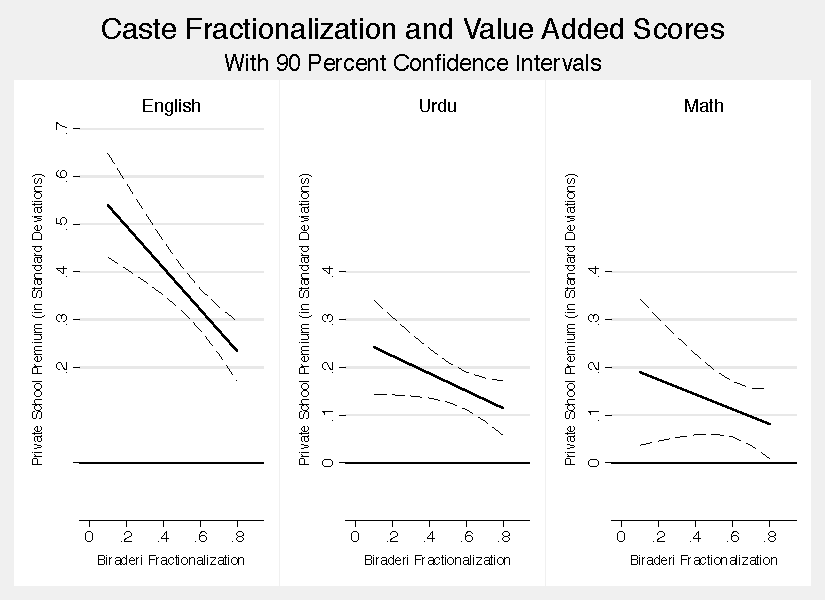
\includegraphics[scale=0.8]{graphs/kids_combined.pdf}
\end{figure}

\begin{sidewaystable}[htbp]\centering
\def\sym#1{\ifmmode^{#1}\else\(^{#1}\)\fi}
\caption{Child Test Scores\label{kids}}
\begin{tabular}{l*{9}{c}}
\toprule
                &\multicolumn{3}{c}{English}           &\multicolumn{3}{c}{Urdu}              &\multicolumn{3}{c}{Math}              \\\cmidrule(lr){2-4}\cmidrule(lr){5-7}\cmidrule(lr){8-10}
                &\multicolumn{1}{c}{(1)}&\multicolumn{1}{c}{(2)}&\multicolumn{1}{c}{(3)}&\multicolumn{1}{c}{(4)}&\multicolumn{1}{c}{(5)}&\multicolumn{1}{c}{(6)}&\multicolumn{1}{c}{(7)}&\multicolumn{1}{c}{(8)}&\multicolumn{1}{c}{(9)}\\
                &\multicolumn{1}{c}{}&\multicolumn{1}{c}{}&\multicolumn{1}{c}{}&\multicolumn{1}{c}{}&\multicolumn{1}{c}{}&\multicolumn{1}{c}{}&\multicolumn{1}{c}{}&\multicolumn{1}{c}{}&\multicolumn{1}{c}{}\\
\midrule
Private School  &     0.63***&     0.60***&     0.59***&     0.27***&     0.26***&     0.20***&     0.19*  &     0.19*  &     0.12   \\
                &   (8.35)   &   (7.28)   &   (7.31)   &   (4.16)   &   (4.01)   &   (2.93)   &   (1.67)   &   (1.88)   &   (1.25)   \\
Fractionalization * Private&    -0.43***&    -0.41***&    -0.42***&    -0.17*  &    -0.17*  &   -0.094   &   -0.082   &    -0.12   &   -0.052   \\
                &  (-3.77)   &  (-3.46)   &  (-3.68)   &  (-1.71)   &  (-1.74)   &  (-0.98)   &  (-0.53)   &  (-0.83)   &  (-0.39)   \\
Lagged English Scores&     0.37***&     0.36***&     0.39***&     0.15***&     0.14***&     0.14***&     0.16***&     0.15***&     0.16***\\
                &  (21.16)   &  (20.03)   &  (20.61)   &  (13.05)   &  (11.37)   &  (11.69)   &  (10.78)   &  (10.06)   &   (9.86)   \\
Lagged Math Scores&    0.069***&    0.072***&    0.071***&     0.12***&     0.12***&     0.12***&     0.37***&     0.38***&     0.40***\\
                &   (8.55)   &   (8.91)   &   (8.49)   &  (14.10)   &  (13.51)   &  (13.96)   &  (29.56)   &  (27.37)   &  (28.76)   \\
Lagged Urdu Scores&     0.15***&     0.15***&     0.15***&     0.38***&     0.38***&     0.40***&     0.23***&     0.22***&     0.22***\\
                &  (14.04)   &  (13.28)   &  (12.71)   &  (34.36)   &  (32.65)   &  (31.74)   &  (17.67)   &  (17.01)   &  (16.84)   \\
Child's Wealth Index&            &    0.017***&    0.015***&            &   0.0073** &   0.0068** &            &    0.014***&    0.016***\\
                &            &   (5.19)   &   (4.29)   &            &   (2.46)   &   (2.28)   &            &   (3.52)   &   (3.73)   \\
Educated Parent &            &    0.058***&    0.053***&            &    0.052***&    0.049***&            &    0.046***&    0.043***\\
                &            &   (4.75)   &   (4.07)   &            &   (4.77)   &   (4.40)   &            &   (3.35)   &   (3.08)   \\
Biraderi Fractionalization&            &            &     0.21** &            &            &    0.095   &            &            &     0.14   \\
                &            &            &   (2.56)   &            &            &   (1.40)   &            &            &   (1.38)   \\
Village: Pct Adults Literate&            &            &  0.00017   &            &            & -0.00054   &            &            &  0.00036   \\
                &            &            &   (0.18)   &            &            &  (-0.62)   &            &            &   (0.27)   \\
Log Village Size&            &            &    0.019   &            &            &    0.014   &            &            &   0.0088   \\
                &            &            &   (1.47)   &            &            &   (1.01)   &            &            &   (0.50)   \\
Village Land Gini&            &            &    0.053   &            &            &    0.061   &            &            &    -0.25*  \\
                &            &            &   (0.47)   &            &            &   (0.63)   &            &            &  (-1.88)   \\
Constant        &     0.25   &     0.40*  &     0.57** &     0.56** &     0.69***&     0.78***&     0.12   &     0.31   &     0.60*  \\
                &   (0.99)   &   (1.78)   &   (2.28)   &   (2.58)   &   (2.78)   &   (2.80)   &   (0.37)   &   (0.99)   &   (1.74)   \\
Village Fixed Effects&      Yes   &      Yes   &       No   &      Yes   &      Yes   &       No   &      Yes   &      Yes   &       No   \\
District Fixed Effects&       No   &       No   &      Yes   &       No   &       No   &      Yes   &       No   &       No   &      Yes   \\
\midrule
Observations    &    37147   &    26141   &    26141   &    37147   &    26141   &    26141   &    37147   &    26141   &    26141   \\
\bottomrule
\multicolumn{10}{l}{\footnotesize Controls for age, age squared, gender, and class omitted from table. Standard errors clustered at village level.}\\
\multicolumn{10}{l}{\footnotesize * p<0.10, ** p<0.05, *** p<0.01}\\
\end{tabular}
\end{sidewaystable}


Consistent results are also found from data at the level of the village, as shown in Table~\ref{villagegap}. As discussed in methodology, the dependent variable in these regressions is the village gap in government-private ``value-added'' scores after controlling for all available observable differences. This adjusted-gap is then regressed on a number of village characteristics. While the results are not quite as strong as when estimated at the level of the child, all three regressions show declines in the government-private gap associated with increasing fractionalization, especially for English. 

\begin{table}[htbp]\centering
\def\sym#1{\ifmmode^{#1}\else\(^{#1}\)\fi}
\caption{Village Level Government-Private Gap\label{villagegap}}
\begin{tabular}{l*{3}{c}}
\toprule
                &\multicolumn{1}{c}{(1)}&\multicolumn{1}{c}{(2)}&\multicolumn{1}{c}{(3)}\\
                &\multicolumn{1}{c}{English}&\multicolumn{1}{c}{Urdu}&\multicolumn{1}{c}{Math}\\
\midrule
Biraderi Fractionalization&    -0.36*  &    -0.18   &    -0.28   \\
                &  (-1.80)   &  (-1.02)   &  (-1.03)   \\
Median Village Wealth&-0.000010   &0.0000096   &-0.000043   \\
                &  (-0.32)   &   (0.34)   &  (-0.97)   \\
Log Village Size&   0.0016   &   -0.033   &    0.019   \\
                &   (0.03)   &  (-0.63)   &   (0.23)   \\
Pct of Adults Literate& -0.00021   &   0.0019   &   0.0047   \\
                &  (-0.06)   &   (0.64)   &   (1.00)   \\
Land Gini       &     0.35   &   -0.084   &     0.32   \\
                &   (1.01)   &  (-0.27)   &   (0.66)   \\
District Fixed Effects&      Yes   &      Yes   &      Yes   \\
\midrule
Observations    &      109   &      109   &      109   \\
\bottomrule
\multicolumn{4}{l}{\footnotesize \textit{t} statistics in parentheses}\\
\multicolumn{4}{l}{\footnotesize * p<0.10, ** p<0.05, *** p<0.01}\\
\end{tabular}
\end{table}


One feature of this result that strongly suggests this is a story about sorting is that there is not aggregate relationship between academic performance and village fractionalization as one would expect if either government schools were performing better or private schools were performing worse. Rather, Table~\ref{kidsnointeract} shows that scores are essentially flat -- English scores are slightly higher in more fractionalized villages in Column 1, but the magnitude of this difference is relatively small, and once more demographic controls are added in Column 2 this effect disappears. No relationship exists for other subjects. 

\begin{sidewaystable}[htbp]\centering
\def\sym#1{\ifmmode^{#1}\else\(^{#1}\)\fi}
\caption{Child Test Scores and Fractionalization \label{kidsnointeract}}
\begin{tabular}{l*{6}{c}}
\toprule
                &\multicolumn{2}{c}{English}&\multicolumn{2}{c}{Urdu} &\multicolumn{2}{c}{Math} \\\cmidrule(lr){2-3}\cmidrule(lr){4-5}\cmidrule(lr){6-7}
                &\multicolumn{1}{c}{(1)}&\multicolumn{1}{c}{(2)}&\multicolumn{1}{c}{(3)}&\multicolumn{1}{c}{(4)}&\multicolumn{1}{c}{(5)}&\multicolumn{1}{c}{(6)}\\
                &\multicolumn{1}{c}{}&\multicolumn{1}{c}{}&\multicolumn{1}{c}{}&\multicolumn{1}{c}{}&\multicolumn{1}{c}{}&\multicolumn{1}{c}{}\\
\midrule
Private School  &     0.31***&     0.29***&     0.14***&     0.14***&     0.11***&    0.087** \\
                &  (10.98)   &  (10.42)   &   (5.74)   &   (5.65)   &   (3.17)   &   (2.58)   \\
Biraderi Fractionalization&     0.13*  &    0.096   &    0.085   &    0.069   &     0.13   &     0.13   \\
                &   (1.70)   &   (1.33)   &   (1.26)   &   (1.08)   &   (1.34)   &   (1.46)   \\
Lagged English Scores&     0.40***&     0.39***&     0.16***&     0.14***&     0.17***&     0.16***\\
                &  (22.32)   &  (21.10)   &  (13.39)   &  (11.90)   &  (10.27)   &   (9.92)   \\
Lagged Math Scores&    0.067***&    0.070***&     0.12***&     0.12***&     0.39***&     0.40***\\
                &   (8.18)   &   (8.37)   &  (14.51)   &  (14.00)   &  (30.92)   &  (28.87)   \\
Lagged Urdu Scores&     0.15***&     0.15***&     0.39***&     0.40***&     0.23***&     0.22***\\
                &  (13.26)   &  (12.80)   &  (34.01)   &  (31.76)   &  (17.96)   &  (16.86)   \\
Village: Pct Adults Literate&  0.00067   &  0.00022   & -0.00018   & -0.00053   &  0.00043   &  0.00036   \\
                &   (0.68)   &   (0.23)   &  (-0.21)   &  (-0.61)   &   (0.31)   &   (0.27)   \\
Log Number of Households&    0.017   &    0.019   &    0.011   &    0.014   &   0.0070   &   0.0087   \\
                &   (1.33)   &   (1.39)   &   (0.73)   &   (1.01)   &   (0.35)   &   (0.50)   \\
Village Land Gini&   0.0097   &    0.045   &    0.013   &    0.059   &    -0.28** &    -0.25*  \\
                &   (0.08)   &   (0.39)   &   (0.13)   &   (0.61)   &  (-2.22)   &  (-1.90)   \\
Child's Wealth Index&            &    0.015***&            &   0.0068** &            &    0.016***\\
                &            &   (4.22)   &            &   (2.27)   &            &   (3.73)   \\
Educated Parent &            &    0.053***&            &    0.049***&            &    0.043***\\
                &            &   (4.13)   &            &   (4.42)   &            &   (3.08)   \\
Constant        &     0.44   &     0.22   &     0.67***&     0.62   &     0.32   &     0.91   \\
                &   (1.57)   &        .   &   (2.65)   &        .   &   (0.87)   &   (0.00)   \\
District Fixed Effects&      Yes   &      Yes   &      Yes   &      Yes   &      Yes   &      Yes   \\
\midrule
Observations    &    37147   &    26141   &    37147   &    26141   &    37147   &    26141   \\
\bottomrule
\multicolumn{7}{l}{\footnotesize \textit{t} statistics in parentheses}\\
\multicolumn{7}{l}{\footnotesize * p<0.10, ** p<0.05, *** p<0.01}\\
\end{tabular}
\end{sidewaystable}



\subsection{Alternative Explanations}\label{}
An alternative explanation for the findings of this paper is not easy to generate. Any such finding would have to explain why fractionalization (a) has a positive impact on government schools, (b) has a negative effect on private schools in English, but (c) has no effect on aggregate test scores. Nevertheless, a few addition results are worth presenting to further rule out the possibility that this pattern of test score convergence is driven by changes in school quality. 

\subsubsection{Government Schools}\label{} 
Government schools in Pakistan are administered at the state level, and are thus relatively insulated from village politics. Nevertheless, it is worth explicitly showing that there is little difference between government schools in villages with high and low fractionalization. Table~\ref{governmentteachers} presents the relationship between village fractionalization and a number of different school and teacher characteristics. Columns 1 through 5 show teachers in high fractionalization villages have better equipped government schools or better trained government teachers. 

\begin{sidewaystable}[htbp]\centering
\def\sym#1{\ifmmode^{#1}\else\(^{#1}\)\fi}
\caption{Government Teacher Characteristics and Village Fractionalization\label{governmentteachers}}
\begin{tabular}{l*{6}{c}}
\toprule
                &\multicolumn{1}{c}{(1)}&\multicolumn{1}{c}{(2)}&\multicolumn{1}{c}{(3)}&\multicolumn{1}{c}{(4)}&\multicolumn{1}{c}{(5)}&\multicolumn{1}{c}{(6)}\\
                &\multicolumn{1}{c}{Days Absent Last Month}&\multicolumn{1}{c}{Female}&\multicolumn{1}{c}{From Village}&\multicolumn{1}{c}{\specialcellc{Teacher English \ Exam Score}}&\multicolumn{1}{c}{\specialcellc{More than Grade \ School Education}}&\multicolumn{1}{c}{\specialcellc{Basic School \\ Facility Index}}\\
\midrule
Biraderi Fractionalization&    -0.67   &    0.048   &     0.13   &     0.19   &    0.092   &     0.45   \\
                &   (0.56)   &   (0.13)   &   (0.19)   &   (0.19)   &   (0.11)   &   (0.68)   \\
\specialcell{Median Village \\\\ Expenditures}& 0.000089   & 0.000031   &-0.000016   & 0.000029   & 0.000016   &-0.000081   \\
                &(0.000077)   &(0.000027)   &(0.000025)   &(0.000022)   &(0.000015)   &(0.000096)   \\
\specialcell{Log Number \\\\ of Households}&   -0.068   &   -0.033   &   -0.082   &   -0.015   &   -0.034** &    -0.24*  \\
                &  (0.096)   &  (0.024)   &  (0.050)   &  (0.036)   &  (0.015)   &   (0.13)   \\
District Fixed Effects&      Yes   &      Yes   &      Yes   &      Yes   &      Yes   &      Yes   \\
\midrule
Observations    &     1335   &     1337   &     1335   &      990   &     1337   &      295   \\
\bottomrule
\multicolumn{7}{l}{\footnotesize Standard errors in parentheses}\\
\multicolumn{7}{l}{\footnotesize * p<0.10, ** p<0.05, *** p<0.01}\\
\end{tabular}
\end{sidewaystable}


\subsubsection{Private Schools}\label{} 

Results are similar for private schools, whose teachers do not appear to differ markedly between villages of high and low fractionalization. Indeed, what differences do exist -- like higher average educations -- should presumably improve test scores in more fractionalized villages. 

\begin{sidewaystable}[htbp]\centering
\def\sym#1{\ifmmode^{#1}\else\(^{#1}\)\fi}
\caption{Private Teacher Characteristics and Village Fractionalization\label{privateteachers}}
\begin{tabular}{l*{6}{c}}
\toprule
                &\multicolumn{1}{c}{(1)}&\multicolumn{1}{c}{(2)}&\multicolumn{1}{c}{(3)}&\multicolumn{1}{c}{(4)}&\multicolumn{1}{c}{(5)}&\multicolumn{1}{c}{(6)}\\
                &\multicolumn{1}{c}{\specialcellc{Days Absent \\ Last Month}}&\multicolumn{1}{c}{Female}&\multicolumn{1}{c}{\specialcellc{Local \\ Teacher}}&\multicolumn{1}{c}{\specialcellc{More than Grade \\ School Educ}}&\multicolumn{1}{c}{\specialcellc{Teacher's \\ English Score}}&\multicolumn{1}{c}{\specialcellc{Basic School \\ Facility Index}}\\
\midrule
Biraderi Fractionalization&    -0.13   &    -0.15   &     0.21   &     0.11   &     0.30   &     0.45   \\
                &   (0.34)   &  (0.096)   &   (0.16)   &  (0.080)   &   (0.19)   &   (0.68)   \\
\specialcell{Median Village \\ Expenditures}&0.0000047   & 0.000032   &0.0000038   &0.0000096   & 0.000038   &-0.000081   \\
                &(0.000061)   &(0.000021)   &(0.000019)   &(0.000016)   &(0.000024)   &(0.000096)   \\
\specialcell{Log Number \\ of Households}&    0.061   &  -0.0067   &   -0.072*  &   -0.030   &    0.038   &    -0.24*  \\
                &   (0.10)   &  (0.022)   &  (0.039)   &  (0.020)   &  (0.033)   &   (0.13)   \\
District Fixed Effects&      Yes   &      Yes   &      Yes   &      Yes   &      Yes   &      Yes   \\
\midrule
Observations    &     4667   &     4675   &     4670   &     4675   &     1041   &      295   \\
\bottomrule
\multicolumn{7}{l}{\footnotesize Standard errors in parentheses}\\
\multicolumn{7}{l}{\footnotesize * \(p<0.10\), ** \(p<0.05\), *** \(p<0.01\)}\\
\multicolumn{7}{l}{\footnotesize All results clustered at the village level.}\\
\end{tabular}
\end{sidewaystable}



\section{Distance}\label{distance}
The changing salience of ethnicity is not the only source of variation that can be leveraged to better understanding the contributions of sorting to the government-private school performance differential. Research in Pakistan has shown that there is a strong ``distance gradient'' with respect to school enrollment -- even controlling for other factors, students (especially girls) are much more likely to attend primary school if a school is close to their home. This relationship not only has a strong impact on overall enrollment, but also school choice. As noted in the LEAPS report, ``there is a dramatic 10 percentage points (30\%) increase in the probability of using a private school \emph{regardless of wealth} when the private school is closer than a public school.''\citep[p.96]{Andrabi:2007we}. 

In settings where the distance to the nearest private school differs from the distance to the nearest government school, this ``distance aversion'' can be thought of as an impediment to efficient sorting. Namely, the larger the additional distance a child must travel to attend a private school, the more likely a student with high unobservable academic potential is to attend their nearby government school instead.  

This prediction can be readily tested using data from the LEAPS survey, which includes GPS data on all schools and households in the LEAPS sample. If it is the case that students are sorting according to academic potential, then conditional on being a government school student, there should exist a positive correlation between test scores and the additional distance a child would have to travel to attend a private school. 

This prediction is tested in Table~\ref{distancescores} below. As shown in Column 1, even when controlling for the absolute distance to the nearest private school and other demographic characteristics, there is moderate evidence of a positive correlation between additional distance to a private school and English test scores, although the coefficient is only significant at the 80\% level. (Note that each child enters these regressions twice, so the sample size is effectively only 400 for government students and 150 for private school students.) The coefficient for private schools, however, is not positive, but given the effective sample size of only 150 this is not entirely surprising. 

\begin{sidewaystable}[htbp]\centering
\def\sym#1{\ifmmode^{#1}\else\(^{#1}\)\fi}
\caption{Test Scores and Relative Distance of Schools\label{distancescores}}
\begin{tabular}{l*{7}{c}}
\toprule
                &\multicolumn{1}{c}{Selection}&\multicolumn{3}{c}{Government School} &\multicolumn{3}{c}{Private School}    \\\cmidrule(lr){2-2}\cmidrule(lr){3-5}\cmidrule(lr){6-8}
                &\multicolumn{1}{c}{(1)}&\multicolumn{1}{c}{(2)}&\multicolumn{1}{c}{(3)}&\multicolumn{1}{c}{(4)}&\multicolumn{1}{c}{(5)}&\multicolumn{1}{c}{(6)}&\multicolumn{1}{c}{(7)}\\
                &\multicolumn{1}{c}{Private School}&\multicolumn{1}{c}{English}&\multicolumn{1}{c}{Math}&\multicolumn{1}{c}{Urdu}&\multicolumn{1}{c}{English}&\multicolumn{1}{c}{Math}&\multicolumn{1}{c}{Urdu}\\
\midrule
Additional Km to Nearest Private&    -0.14** &    0.096   &    0.018   &    0.058   &    -0.18   &    -0.25   &    -0.17   \\
                &  (-2.40)   &   (1.19)   &   (0.19)   &   (1.02)   &  (-0.80)   &  (-0.98)   &  (-0.66)   \\
Km to Nearest Private Sch&   -0.050   &   -0.043   &    0.018   &   -0.022   &     0.23   &     0.18   &   -0.054   \\
                &  (-1.23)   &  (-0.88)   &   (0.30)   &  (-0.52)   &   (1.41)   &   (0.63)   &  (-0.32)   \\
Log HH Expenditures&    0.014   &   -0.090*  &    -0.11   &   -0.068   &     0.14** &     0.14   &     0.11*  \\
                &   (0.31)   &  (-1.84)   &  (-1.65)   &  (-1.33)   &   (2.04)   &   (1.42)   &   (1.77)   \\
Child Age       &   -0.076   &   -0.019   &    -0.35*  &    -0.11   &    -0.25   &    -0.48   &   -0.084   \\
                &  (-0.56)   &  (-0.14)   &  (-1.78)   &  (-0.82)   &  (-0.86)   &  (-1.39)   &  (-0.36)   \\
Age Squared     &   0.0047   &   0.0019   &    0.015*  &   0.0043   &    0.010   &    0.020   &   0.0039   \\
                &   (0.73)   &   (0.35)   &   (1.91)   &   (0.83)   &   (0.87)   &   (1.46)   &   (0.41)   \\
Mom Educated    &     0.24** &     0.10   &     0.24** &    0.024   &    0.063   &   -0.026   &    0.034   \\
                &   (2.56)   &   (1.18)   &   (2.12)   &   (0.29)   &   (0.58)   &  (-0.21)   &   (0.36)   \\
Dad Educated    &    0.076   &    0.079   &   -0.020   &    0.088*  &    0.040   &     0.26** &    0.033   \\
                &   (1.19)   &   (1.24)   &  (-0.19)   &   (1.73)   &   (0.54)   &   (2.29)   &   (0.36)   \\
Female          &   -0.098   &     0.21***&    -0.31***&     0.14** &   -0.069   &    -0.21*  &   -0.014   \\
                &  (-1.65)   &   (3.03)   &  (-3.21)   &   (2.56)   &  (-0.80)   &  (-1.78)   &  (-0.15)   \\
Lagged Math Scores&            &    0.059** &     0.31***&     0.11** &   -0.010   &    -0.11   &    -0.16   \\
                &            &   (2.00)   &   (4.89)   &   (2.53)   &  (-0.07)   &  (-0.90)   &  (-1.39)   \\
Lagged Urdu Scores&            &     0.13** &     0.24***&     0.32***&     0.17   &     0.12   &     0.32***\\
                &            &   (2.58)   &   (2.72)   &   (4.69)   &   (1.29)   &   (0.73)   &   (2.92)   \\
Lagged English Scores&            &     0.32***&     0.16** &     0.16***&    0.072   &     0.35*  &     0.15   \\
                &            &   (4.81)   &   (2.42)   &   (3.65)   &   (0.98)   &   (1.81)   &   (1.53)   \\
Constant        &     0.39   &   -0.021   &     2.73** &     0.90   &     1.46   &     2.22   &     1.11   \\
                &   (0.51)   &  (-0.03)   &   (2.00)   &   (0.98)   &   (0.73)   &   (0.88)   &   (0.69)   \\
Village Fixed Effects&      Yes   &      Yes   &      Yes   &      Yes   &      Yes   &      Yes   &      Yes   \\
\midrule
Observations    &      483   &      904   &      904   &      904   &      329   &      329   &      329   \\
\bottomrule
\multicolumn{8}{l}{\footnotesize \textit{t} statistics in parentheses}\\
\multicolumn{8}{l}{\footnotesize * p<0.10, ** p<0.05, *** p<0.01}\\
\end{tabular}
\end{sidewaystable}



\section{External Validity}\label{}
\begin{table}[htbp]\centering
\def\sym#1{\ifmmode^{#1}\else\(^{#1}\)\fi}
\caption{India: Child Reading Skills and Fractionalization\label{indiareading}}
\begin{tabular}{l*{3}{c}}
\toprule
                &\multicolumn{1}{c}{(1)}&\multicolumn{1}{c}{(2)}&\multicolumn{1}{c}{(3)}\\
                &\multicolumn{1}{c}{Read Letters}&\multicolumn{1}{c}{Read Sentence}&\multicolumn{1}{c}{Read Story}\\
\midrule
Private School  &    0.082** &     0.19***&     0.13** \\
                &   (2.57)   &   (3.82)   &   (2.15)   \\
Village Fractionalization&    0.021   &    0.050   &    0.046   \\
                &   (0.59)   &   (1.00)   &   (1.07)   \\
Village Frac * Private&   0.0084   &   -0.030   &    0.090   \\
                &   (0.21)   &  (-0.49)   &   (1.19)   \\
Female          &   -0.049***&    -0.11***&    -0.11***\\
                & (-10.55)   & (-15.70)   & (-16.07)   \\
Child Age       &     0.18***&     0.26***&     0.15***\\
                &  (14.97)   &  (16.12)   &  (11.64)   \\
Child Age Squared&  -0.0069***&  -0.0087***&  -0.0031***\\
                & (-13.04)   & (-12.05)   &  (-5.27)   \\
\midrule
Observations    &    31703   &    31703   &    31703   \\
\bottomrule
\multicolumn{4}{l}{\footnotesize Each model regressions a dummy for given ability against controls}\\
\multicolumn{4}{l}{\footnotesize * p<0.10, ** p<0.05, *** p<0.01}\\
\end{tabular}
\end{table}

\begin{table}[htbp]\centering
\def\sym#1{\ifmmode^{#1}\else\(^{#1}\)\fi}
\caption{India: Child Math Skills and Fractionalization\label{indiamath}}
\begin{tabular}{l*{3}{c}}
\toprule
                &\multicolumn{1}{c}{(1)}&\multicolumn{1}{c}{(2)}&\multicolumn{1}{c}{(3)}\\
                &\multicolumn{1}{c}{Read Numbers}&\multicolumn{1}{c}{Subtraction}&\multicolumn{1}{c}{Division}\\
\midrule
Private School  &     0.17***&     0.16***&     0.11** \\
                &   (3.15)   &   (3.33)   &   (2.31)   \\
Village Fractionalization&    0.010   &    0.069   &    0.085***\\
                &   (0.18)   &   (1.37)   &   (3.19)   \\
Village Frac * Private& -0.00036   &    0.013   &    0.021   \\
                &  (-0.01)   &   (0.20)   &   (0.33)   \\
Female          &    -0.19***&    -0.22***&    -0.19***\\
                & (-25.83)   & (-32.76)   & (-34.18)   \\
Child Age       &     0.24***&     0.14***&    0.079***\\
                &  (16.05)   &  (11.62)   &   (7.59)   \\
Child Age Squared&  -0.0080***&  -0.0041***&  -0.0017***\\
                & (-11.96)   &  (-7.31)   &  (-3.53)   \\
\midrule
Observations    &    31703   &    31703   &    31703   \\
\bottomrule
\multicolumn{4}{l}{\footnotesize Each model regressions a dummy for given ability against controls}\\
\multicolumn{4}{l}{\footnotesize * p<0.10, ** p<0.05, *** p<0.01}\\
\end{tabular}
\end{table}

\section{Conclusion}\label{conclusion}
The results presented here are unlikely to end the debate over the social value of private schools in Pakistan, but they do provide strong evidence that significant skepticism is warranted when using even extremely high quality observational test score data.

\pagebreak

	\bibliography{/Users/Nick/Dropbox/Dropbox_Documents/my_library}
	\bibliographystyle{apalike}

\pagebreak

\appendix


\section{Appendix}\label{biraderis}

[Summary of biraderis here]

\end{document}